\documentclass[12pt]{report} % Increased the font size to 12pt
\usepackage{epigraph}
\usepackage{geometry}

% Optional: customize the style of epigraphs
\setlength{\epigraphwidth}{0.5\textwidth} % Adjust the width of the epigraph
\renewcommand{\epigraphflush}{flushright} % Align the epigraph to the right
\renewcommand{\epigraphrule}{0pt} % No horizontal rule
\usepackage[most]{tcolorbox}
\usepackage{amsmath, amssymb, amsthm}
\usepackage{graphicx}
\usepackage{caption}
\usepackage[utf8]{inputenc}
\usepackage{hyperref} % Added for hyperlinks
\usepackage{listings} % Added for code listings
\usepackage{color}    % Added for color definitions
\usepackage[super]{nth} 
\usepackage{fancyhdr}
\usepackage{tikz}
\usepackage{cite}
\usetikzlibrary{shapes.geometric, arrows, positioning}

\tikzstyle{startstop} = [rectangle, rounded corners, minimum width=3cm, minimum height=1cm, text centered, draw=black, fill=red!30]
\tikzstyle{io} = [trapezium, trapezium left angle=70, trapezium right angle=110, minimum width=3cm, minimum height=1cm, text centered, draw=black, fill=blue!30]
\tikzstyle{process} = [rectangle, minimum width=3cm, minimum height=1cm, text centered, draw=black, fill=orange!30]
\tikzstyle{decision} = [diamond, minimum width=3cm, minimum height=1cm, text centered, draw=black, fill=green!30]
\tikzstyle{arrow} = [thick,->,>=stealth]

% Define the graphics path
%\graphicspath{{./Plots/}}

% Define the header and footer for general pages
\pagestyle{fancy}
\fancyhf{} % Clear all header and footer fields
\fancyhead{} % Initially, the header is empty
\fancyfoot[C]{\thepage} % Page number at the center of the footer
\renewcommand{\headrulewidth}{0pt} % No header line on the first page of chapters
\renewcommand{\footrulewidth}{0pt} % No footer line

% Define the plain page style for chapter starting pages
\fancypagestyle{plain}{%
  \fancyhf{} % Clear all header and footer fields
  \fancyfoot[C]{\thepage} % Page number at the center of the footer
  \renewcommand{\headrulewidth}{0pt} % No header line
}

% Apply the 'fancy' style to subsequent pages in a chapter
\renewcommand{\chaptermark}[1]{%
  \markboth{\MakeUppercase{#1}}{}%
}

% Redefine the 'plain' style for the first page of chapters
\fancypagestyle{plain}{%
  \fancyhf{}%
  \fancyfoot[C]{\thepage}%
  \renewcommand{\headrulewidth}{0pt}%
}

% Header settings for normal pages (not the first page of a chapter)
\fancyhead[L]{\slshape \nouppercase{\leftmark}} % Chapter title in the header
\renewcommand{\headrulewidth}{0.4pt} % Header line width on normal pages

\setlength{\headheight}{14.49998pt}
\addtolength{\topmargin}{-2.49998pt}
% Define colors for code listings
\definecolor{codegreen}{rgb}{0,0.6,0}
\definecolor{codegray}{rgb}{0.5,0.5,0.5}
\definecolor{codepurple}{rgb}{0.58,0,0.82}
\definecolor{backcolour}{rgb}{0.95,0.95,0.92}

% Setup for code listings
\lstdefinestyle{mystyle}{
    backgroundcolor=\color{backcolour},   
    commentstyle=\color{codegreen},
    keywordstyle=\color{magenta},
    numberstyle=\tiny\color{codegray},
    stringstyle=\color{codepurple},
    basicstyle=\ttfamily\footnotesize,
    breakatwhitespace=false,         
    breaklines=true,                 
    captionpos=b,                    
    keepspaces=true,                 
    numbers=left,                    
    numbersep=5pt,                  
    showspaces=false,                
    showstringspaces=false,
    showtabs=false,                  
    tabsize=2
}

\lstset{style=mystyle}

% Definition of the tcolorbox for definitions
\newtcolorbox{definitionbox}{
  colback=red!5!white,
  colframe=red!75!black,
  colbacktitle=red!85!black,
  title=Definition:,
  fonttitle=\bfseries,
  enhanced,
}

% Definition of the tcolorbox for remarks
\newtcolorbox{remarkbox}{
  colback=blue!5!white,     % Light blue background
  colframe=blue!75!black,   % Darker blue frame
  colbacktitle=blue!85!black, % Even darker blue for the title background
  title=Remark:,            % Title text for remark box
  fonttitle=\bfseries,      % Bold title font
  enhanced,
}

% Definition of the tcolorbox for examples
\newtcolorbox{examplebox}{
  colback=green!5!white,
  colframe=green!75!black,
  colbacktitle=green!85!black,
  title=Example:,
  fonttitle=\bfseries,
  enhanced,
}

% Definitions and examples will be put in these environments
\newenvironment{definition}
    {\begin{definitionbox}}
    {\end{definitionbox}}

\newenvironment{example}
    {\begin{examplebox}}
    {\end{examplebox}}

\geometry{top=1.5in} % Adjust the value as needed
% ----------------------------------------------------------------------------------------


\title{S1 Principles of Data Science Coursework Report}
\author{CRSiD: tmb76}
\date{University of Cambridge}

\begin{document} 

\maketitle

\section*{Section A}

\subsection*{(a)}

We have the continuous random variable $M \in{[5;5.6]}$. Our model is the weighted sum of a background and signal such that:  


\begin{equation}
p(M;f,\lambda,\mu,\sigma) = fs(M;\mu,\sigma) + (1 - f)b(M;\lambda)
\end{equation}
where:
\begin{center}
$s(M;\mu,\sigma) = \frac{1}{\sqrt{2\pi}\sigma} e^{-\frac{{(M - \mu)}^{2}}{2\sigma^{2}}}$
\end{center}
\begin{center}
$b(M;\lambda) = \lambda e^{-\lambda M}$
\end{center}
\vspace{1\baselineskip}  
We want to show that:  
\begin{equation}
I = \int_{-\infty}^{+\infty} p(M;f,\lambda,\mu,\sigma)\, dM = 1
\end{equation}
We have:  

\vspace{1\baselineskip}  
$I = \displaystyle\int_{-\infty}^{+\infty} fs(M;\mu,\sigma) + (1-f)b(M;\lambda), dM$  

$I = \displaystyle\int_{-\infty}^{+\infty} f\frac{1}{\sqrt{2\pi}\sigma} e^{-\frac{{(M - \mu)}^{2}}{2\sigma^{2}}}\, dM +  \displaystyle\int_{0}^{+\infty} (1-f)\lambda e^{-\lambda M}\, dM$  

\vspace*{1\baselineskip}
Since the exponential decay distribution is only defined from 0 to $+\infty$. We can first evaluate the 2\textsuperscript{nd} integral:  

\vspace*{1\baselineskip}
$\displaystyle \int_{0}^{+\infty} (1-f)\lambda e^{-\lambda M}\, dM  =  (1-f){[-e^{-\lambda M}]}_{0}^{\infty}  =  (1-f)[0 - (-1)]  =  (1-f)$  

\vspace*{1\baselineskip}
Then, we evaluate the integral of the signal part of the model, taking the $f$ weight out. We use a change of variable so that $u = \frac{(M-\mu)}{\sigma} \iff du = \sigma dM$, thus:

\vspace*{1\baselineskip}
$J = \displaystyle \int_{-\infty}^{+\infty} \frac{1}{\sqrt{2\pi}\sigma} e^{-\frac{{(M - \mu)}^{2}}{2\sigma^{2}}}\, dM = \displaystyle \int_{-\infty}^{+\infty} \frac{1}{\sqrt{2\pi}} e^{-\frac{{(u)}^{2}}{2}}\, du$  

\vspace*{1\baselineskip}
We can square multiply this integral by itself, using dummy variables x and y:  

\vspace*{1\baselineskip}
$J^{2} = \displaystyle \int_{-\infty}^{+\infty} \frac{1}{\sqrt{2\pi}} e^{-\frac{{(x)}^{2}}{2}}\, dx \times \displaystyle \int_{-\infty}^{+\infty} \frac{1}{\sqrt{2\pi}} e^{-\frac{{(y)}^{2}}{2}}\, dy$  

$J^{2} = \frac{1}{2\pi}\displaystyle \int_{-\infty}^{+\infty} \int_{-\infty}^{+\infty}  e^{-\frac{{(x)}^{2}}{2}} e^{-\frac{{(y)}^{2}}{2}}\, dx \, dy$  

$J^{2} = \frac{1}{2\pi}\displaystyle \int_{-\infty}^{+\infty} \int_{-\infty}^{+\infty} e^{-\frac{1}{2}(x^{2}+y^{2})}\, dx \, dy$  

\vspace*{1\baselineskip}
From here, we can switch to polar coordinates to be able to evaluate this. We have $x = r\cos{(\theta)} y = r\sin{(\theta)}$. This means we need to change the limits to polar equivalents. We will get $r \in{[0,\infty]}$ and $\theta \in{[0,2\pi]}$. Further, $dx dy = r dr d\theta$:  

\vspace*{1\baselineskip}
$J^{2} = \frac{1}{2\pi}\displaystyle \int_{0}^{2\pi} \int_{0}^{+\infty} e^{-\frac{1}{2}r^{2}}r\, dr \, d\theta$  

$J^{2} = \frac{1}{2\pi}\displaystyle \int_{0}^{2\pi} {[-e^{-\frac{1}{2}r^{2}}]}_{0}^{\infty}\, d\theta$  

$J^{2} = \frac{1}{2\pi}\displaystyle \int_{0}^{2\pi} [-0 - (-1)]\, d\theta$  

$J^{2} = \displaystyle \frac{1}{2\pi}\displaystyle \int_{0}^{2\pi} 1\, d\theta$  

$J^{2} = \displaystyle \frac{1}{2\pi}\displaystyle {[\theta]}_{0}^{2\pi}$  

$J^{2} = \displaystyle \frac{1}{2\pi}\displaystyle {[2\pi - 0]}$  

$J^{2} = 1$ 

\vspace*{1\baselineskip}
This then means that $J = \pm 1$ but since $s(M;\mu,\sigma) > 0 \forall M \in [-\infty,\infty]$, $ J = 1$. Thus: $I = (1-f) + f = 1$.  


\subsection*{(b)}
We want to find an expression of $p(M;\vec{\theta})$ such that it is normalised between $\alpha$ and $\beta$. Now because the signal fraction $f$ is such that:

\begin{equation}
    \frac{f \times s(M;\mu,\sigma)}{(1 - f)\times b(M;\lambda)} = \frac{f}{1-f}
\end{equation}

This means that we need to normalise the signal and background components separately. This gives:

\begin{equation}
    \displaystyle \int_{\alpha}^{\beta} f N_{s} \times s(M;\mu,\sigma) + (1 - f)N_{b} \times b(M;\lambda)\, dM = 1
\end{equation}  

with:

\begin{equation}
    \frac{1}{N_{s}} = \displaystyle \int_{\alpha}^{\beta} s(M;\mu,\sigma)\, dM
\end{equation}

\begin{equation}
    \frac{1}{N_{b}} = \displaystyle \int_{\alpha}^{\beta} b(M;\lambda)\, dM.
\end{equation}

\vspace*{1\baselineskip}
where $N_{s}$ and $N_{b}$ are a function of parameters $\vec{\theta}$. Now, from the definition of the Cumulative Distribution Function (c.d.f.): $F(X') = \int_{-\inf}^{X'} f(X)\, dX$, where $X'$ is a specific value of the random variable $X$, and $f(X)$ is the p.d.f.(The lower limit is 0 for the exponential decay distribution)\cite[pp. 20-24]{Wass}. This means we can write (5) and (6) as:

\begin{equation}
    \frac{1}{N_{s}} = \displaystyle \int_{\alpha}^{\beta} s(M;\mu,\sigma)\, dM = F_{s}(\beta) - F_{s}(\alpha)
\end{equation}

\begin{equation}
    \frac{1}{N_{b}} = \displaystyle \int_{\alpha}^{\beta} b(M;\lambda)\, dM = F_{b}(\beta) - F_{b}(\alpha)
\end{equation}

\vspace*{1\baselineskip}
We know that the normal and exponential decay distributions have:  

\begin{equation}
    Normal: \displaystyle F(X) = \frac{1}{2}[1 + erf(\frac{X - \mu}{\sigma\sqrt{2}})]
\end{equation}  

\begin{equation}
    Exponential\ Decay: \displaystyle F(X) = 1 - e^{-\lambda X}
\end{equation}  

\vspace*{1\baselineskip}
From equation (7) and (8), we can write the normalisation factors as:

\begin{equation}
    \frac{1}{N_{s}} = \frac{1}{2}[1 + erf(\frac{\beta - \mu}{\sigma\sqrt{2}})] - \frac{1}{2}[1 + erf(\frac{\alpha - \mu}{\sigma\sqrt{2}})] = \frac{1}{2}[erf(\frac{\beta - \mu}{\sigma\sqrt{2}}) - erf(\frac{\alpha - \mu}{\sigma\sqrt{2}})]
\end{equation}

\begin{equation}
    \frac{1}{N_{b}} = (1 - e^{-\lambda \beta}) - (1 - e^{-\lambda \alpha}) = e^{-\lambda \alpha} - e^{-\lambda \beta}
\end{equation}

\vspace*{1\baselineskip}
Finally, this gives the total p.d.f.\ of the model as:

\begin{equation}
    p(M;\vec{\theta}) = \frac{f}{2}[erf(\frac{\beta - \mu}{\sigma\sqrt{2}}) - erf(\frac{\alpha - \mu}{\sigma\sqrt{2}})] \times s(M;\mu,\sigma) + (1 - f)[e^{-\lambda \alpha} - e^{-\lambda \beta}] \times b(M;\lambda)
\end{equation}

\subsection*{(c)}

In this question, we check that the integral of the p.d.f.\ between $\alpha$ and $\beta$ does equal unity. For this specific case, the \texttt{scipy.integrate} library \cite{scipy-integrate} is used to numerically integrate the component-wise normalised p.d.f.\ as described in equation (4). Though $N_{s}$ and $N_{b}$, are computed using the \texttt{scipy.integrate} library \cite{scipy-integrate}, like in (5) and (6). The components are computed using \texttt{scipy.stats} library's \texttt{norm.pdf} and \texttt{expon.pdf} methods \cite{scipy-stats} (cf.\ \texttt{funcs.py} file; \texttt{pdf\_norm}, \texttt{signal\_norm}, \texttt{background\_norm} function). Then, the weighted sum of the two is computed. Finally, that p.d.f.\ is integrated from $\alpha$ to $\beta$, with randomly generated $\vec{\theta}$ parameters, using \texttt{random.uniform} \cite{python-random}. The results are shown in the table below:

\begin{center}
    \begin{table}[htbp]
        \begin{tabular}{ |c|c|c|c|c| } 
            \hline
            $\mu$ & $\sigma$ & $\lambda$ & $f$ & $Integral$ \\ 
            \hline
            5.2357 & 0.0190 & 0.3643 & 0.5044 & 1.0 \\ 
            \hline
            5.5436 & 0.0105 & 0.3823 & 0.6081 & 1.0 \\ 
            \hline
            5.3184 & 0.0214 & 0.6424 & 0.6882 & 1.0 \\ 
            \hline
            5.3621 & 0.0221 & 0.3695 & 0.3625 & 1.0 \\ 
            \hline
            5.3640 & 0.0231 & 0.5015 & 0.2442 & 1.0 \\ 
            \hline
        \end{tabular}
        \centering
        \caption{Results for different values of $\vec{\theta}$ parameters.\ (cf.\ \texttt{solve\_part\_c.py} file)}
    \end{table}
\end{center}

\subsection*{(d)}

For this question, the true values of the parameters were set and used to plot the p.d.f.\ of the model, along with the signal and background component overlayed. The parameters are assumed to be:

\begin{center}
    $\mu = 5.28$;  
    $\sigma = 0.018$; 
    $\lambda = 0.5$; 
    $f = 0.1$
\end{center}

The \texttt{signal\_norm}, \texttt{background\_norm}, and \texttt{pdf\_norm} functions, described in (c) were used to compute the p.d.f.\ of the model, signal, and background, normalised for $M\in{[5,5.6]}$. The results are shown in the figure below:

\newpage

\begin{figure}[htbp]
    \centering
    \includegraphics[width=\textwidth]{../plots/plot_pdf_d_comp.png}
    \captionsetup{margin=1.3cm}
    \caption[width=0.2\pdfpagewidth]{Plot of the total p.d.f.\ of the model, scaled signal and background, normalised for $M\in{[5,5.6]}$.}
\end{figure}  

It is worth keeping in mind the importance of the $f$ weight here. Figure 1 shows the scaled signal, which here means scaling by 0.1. In other words the signal component would be 10 times larger than this if $f=1$.

\subsection*{(e)}

The ``true'' p.d.f., signal and background component are now known and have been visualised (Fig. 1). The context is now to generate a dataset from this ``true'' p.d.f., and to assume this is an observed sample obtained in an experiment. From this sample, the goal is now to try and estimate these ``true'' parameters, using a chosen estimation method.  

To generate the sample, an accept-reject method was used\cite{wiki-rejection-sampling}. The accept-reject method requires us to know the p.d.f.\ function over the $M$ domain, and the maximum value of the p.d.f.\ in the $M$ domain, $y_{\max}$. Uniformly random values of $M$ between $\alpha$ and $\beta$ are generated, using \texttt{random.uniform}\cite{python-random}. Then, for each of these values, many uniform random values of $y$ are generated between 0 and $y_{\max}$. If these generated $y$'s are such that $y \leq p(M;\vec{\theta})$ for the generated $M$ then the \textbf{$\mathbf{M}$ value} is accepted and added to the sample. This is repeated until the sample size is reached (cf.\ \texttt{funcs.py} file, \texttt{accept\_reject} function).  

The chosen estimation method is the Maximum Likelihood Estimation (MLE) method\cite[pp. 122-128]{Wass}. This method relies on the likelihood function, which stands for the probability of observing the data given a set of parameters and is defined as:

\begin{equation}
    \mathcal{L}(\vec{\theta}) = \displaystyle \prod_{i=1}^{N} p(M_{i};\vec{\theta})
\end{equation}

It is a function of the parameters $\vec{\theta}$ only. The goal of the MLE method is to find estimates of the parameters $\vec{\theta}$ that maximise the likelihood function\cite[pp. 122-128]{Wass}. In other words, finding $\vec{\hat{\theta}}$, such that:  

\begin{equation}
    \frac{\delta\mathcal{L}(\vec{\hat{\theta}})}{\delta \theta} = 0
\end{equation}

This result is because maximising the probability of observing $M$ given a certain set $\vec{\hat{\theta}}$ means we have found the set of parameters $\vec{\hat{\theta}}$ that are the most likely to be the ones the data was observed under. Now because summing small numbers is less of a problem as multiplying small numbers in computations, we take the logarithm of the likelihood function, to turn the product into a sum. And taking twice the negative of that gives a negative log-likelihood function:

\begin{equation}
    -2\ln{\mathcal{L}(\vec{\theta})} = -2\displaystyle \sum_{i=1}^{N} \ln{p(M_{i};\vec{\theta})}
\end{equation}

And this is the function to now \textbf{minimise}. To do so we use a python package named \texttt{iminuit}\cite{iminuitBasics}, which possesses a very useful set of minimising tools. The \texttt{iminuit} package requires a function to minimise, called a cost function, and a set of initial guesses for the parameters. Luckily, \texttt{iminuit} possesses a series of standard cost functions\cite{iminuitCOST}. The one used here is the \texttt{BinnedNLL}, Binned Negative Log-Likelihood, which takes in the c.d.f.\ of a \textbf{normalised} probability density and the observed \textbf{binned} data we want to fit that density to. With the cost function defined, \texttt{iminuit}'s main function \texttt{Minuit}\cite{iminuitMinuit}, a function minimizer and error computer, takes that cost function in along with initial guesses for the parameters. These initial guesses are usually educated guesses at what the true parameters may be. Then we call the \texttt{migrad} method, which is a gradient descent method, to conduct the minimization\cite{iminuitMigrad}.

An important point is that \texttt{iminuit.Minuit} reads the function given in the cost function definition to read the parameters it needs to fit for. In other words, using the \texttt{pdf\_norm} function from (d), \texttt{Minuit.migrad()} would minimise the cost function for the $\vec{\theta}$ parameters as well as $\alpha$ and $\beta$\cite{iminuitBasics}.

Furthermore, in the interest of performance, the \texttt{numba\-stats} library\cite{numba-stats} was used to speed up any computation that uses our new p.d.f.\ function. This library provides \texttt{numba}-accelerated statistical function for common probability distributions, mostly following \texttt{scipy.stats} library's conventions\cite{scipy-stats}. So the c.d.f.\ of the model was defined to only take the $\vec{\theta}$ parameters. It then uses the \texttt{numba\_stats.truncnorm.cdf} and \texttt{.truncexpon.cdf} functions. Running the minimisation, the following parameter estimates and their uncertainties were obtained:  

\begin{center}
    $\hat{\mu} = 5.27939 \pm 0.00033$;  

    $\hat{\sigma} = 0.01820 \pm 0.0032$;  
    
    $\hat{\lambda} = 0.490 \pm 0.019$;  

    $\hat{f} = 0.1008 \pm 0.0017$
\end{center}

We can see that the minimisation performed well, with close estimates and relatively small uncertainties. Those uncertainties were obtained using a Hessian matrix. By taking the inverse of the Hessian matirx, the matrix of 2$^{nd}$ derivatives of the cost function for all free parameters, one can approximate the covariance matrix. Then, taking the diagonal elements gives an approximation of the variance of the estimates. Taking the squareroot gives the standard deviation. With those parameter estimates, the following plot of the data and the fitted model was obtained:

\begin{figure}[tp]
    \centering
    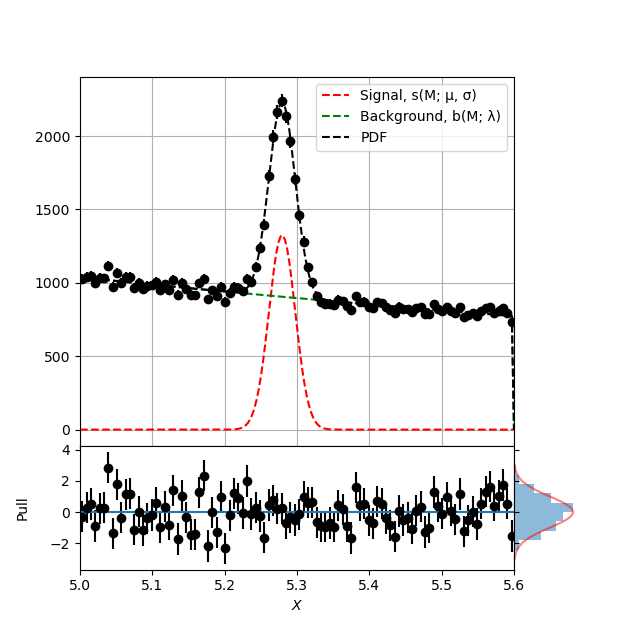
\includegraphics[width=\textwidth]{../plots/plot_pdf_e.png}
    \captionsetup{margin=1.3cm}
    \caption[width=0.2\pdfpagewidth]{Plots of the binned data, with uncertainties defined by the Poisson distribution ($\sqrt{N}$) and the fitted signal, background, and total p.d.f. model from the estimated parameters (top). And of the pull values for each bin, with their distribution histogram on the right (bottom).}
\end{figure}

\newpage

The lower plots are plots of the pull: $pull = \frac{obs - pred}{\sqrt{N}}$, where $N$ is the bin counts. In other words, they are the errors weighted by the uncertainties. The pull plots are a good way to check that the uncertainties are sensible, and is also known as the student's t-distribution\cite{Haslwanter2022}. Figure 2 shows an agreement between the original data and the fitted model, with the pull values being approximately normally distributed around 0, as expected. Comparing with Figure 1, we also see that our generated data is sensible and not entirely different to the ``true'' model.


\section*{Section B}

\subsection*{(f) and (g)}

\subsubsection*{Introduction}
In this section, the context is now the discovery of a signal in an observed dataset, similar to searching for a particle using a collider\cite{kenzie2014properties}. To classify the signal as discovered, a significance of at least 5 standard deviations of a normal distribution. Let's imagine there is a search for a particle going on and, obviously, data needs to be collected. However, the more data we need to collect, the more expensive the running of the experiment becomes.  

The task at hand is to simulate the experiment numerically and find the smallest possible dataset size for which the signal is discovered at least 90\% of the time. To do this, a hypothesis test can be conducted with the null hypothesis being that there is only background being observed in our data, and the alternate hypothesis being that there is one signal on top of the background\cite[p. 164]{Wass}. The second task is a similar one, but this time, the experiment is expected to reveal 2 signals in the data. Again, the goal is to find the smallest possible dataset size for which the 2 signals instead of 1 are discovered at least 90\% of the time. This means the null hypothesis will be that there is only one signal on top of the background, and the alternate hypothesis will be that there are in fact 2 of them. In the context of hypthesis testing, the discovery threshold can be defined as the p-value with which we can make a decision regarding the null hypothesis\cite[p. 164]{Wass}.

\subsubsection*{Method}

\underline{For (f):}  

\vspace*{1\baselineskip}
The general idea is to generate many pretend datsets for multiple sample sizes and conduct hypothesis testing on each of them to obtain a p-value, for which we can confidently reject the null hypothesis, i.e.\ at our discovery threshold ($2.9 \times 10^{-7}$).  
First, a very large dataset (100,000 samples) is generated, from the same p.d.f.\ as in (e), with the same ``true'' parameters using the previously described accept-reject method. Sample sizes to test are generated as a base-10 logarithmic scale from 100 to 10000. For each sample size, 1000 datasets are generated by bootstrapping from the larger dataset.


Bootstrapping is a resampling method that consists of sampling with replacement from a dataset to create a new dataset of the same size, or smaller. When doing so from a model, it is called parametric bootstrapping, and can be referred to as ``throwing toys'' or generating pretend datasets. One other use is to estimate parameters and their uncertainties, by estimating them for each toy and taking the mean and standard deviation of the resulting distributions\cite[p. 108]{Wass}.  

In this simulation, for each bootstrapped sample, a hypothesis test is conducted. The test is set up with the null hypothesis being that there is only background being observed in our data, and the alternate hypothesis being that there is one signal on top of the background. In other words:  

\begin{center}
    $H_{0}: p(M;\vec{\theta}) = b(M;\lambda)$  

    \vspace*{1\baselineskip}  
    $H_{1}: p(M;\vec{\theta}) = fs(M;\mu,\sigma) + (1 - f)b(M;\lambda)$
\end{center}

It can be seen that the null hypothesis is simply the case where $f=0$. Just like when determining the profiled log-likelihood, the parameter can be fixed, and the likelihood function minimised for all other parameters. $f$ can be set to 0, and the negative log-likelihood minimised for $\mu$, $\sigma$, and $\lambda$. This is possible to do when setting up \texttt{Minuit}, $f$ can be fixed at 0, while all other parameters are allowed to float. Then, running \texttt{migrad} will minimise the cost function for all other parameters. Then, a second instance of \texttt{Minuit} is set up, where $f$ is now allowed to float, just like in (e), and run \texttt{migrad} again\cite{iminuitMinuit}\cite{iminuitMigrad}.  

Doing so, 2 hypothesis are being fitted to the samples, and we can obtain the minimum negative log-likelihood values for each of those fits\cite{iminuitmethod}. Now the hypothesis test relies on a chosen test statistic. The test statistic used here is the difference between the 2 minimised negative log-likelihood values under each hypothesis, or the negative log-likelihood ratio:

\begin{equation}
    T = -2 \ln{\frac{\mathcal{L}(f = 0)}{\mathcal{L}(f = \hat{f})}}
\end{equation}

The reason this test is used is backed up by the Neyman-Pearson Lemma, which asserts that a test statistic of this form has the strongest statistical power, for any test size. In other words, it maximises the critical region, under the test-statistic's distribution curve, whose area is the value for which a decision regarding the alternate hypothesis can be made\cite[p. 170]{Wass}. Now, from Wilk's theorem, this test-statistic will be approximately distributed as a $\chi^{2}$ with number of degrees of freedom (DoF), the difference in the number of free parameters under the alternate and the null hypotheses\cite{Wilkls1938}. Wilk's theorem applies here because the hypothesis test has been set up so that the null is a subset case of the alternate\cite{huelsenbeck1997phylogeny}.  

To give more confidence to this result, a side simulation was run, to fit the T-statistic distribution with a $\chi^{2}$ and determine the number of DoF. Similar to (e), but with a dataset generated from the null hypothesis, i.e.\ $f=0$. By bootstrapping from it, a distribution of the test-statistic under the null hypothesis is obtained. Using \texttt{iminuit}, and defining the cost function as the unbinned NLL of the $\chi^{2}$ distribution p.d.f., we fit for the number of DoF parameter for that observed distribution\cite{iminuitmethod}. It is worth to note that this simulation encountered a number of issues, including problems with non-valid operations due to \texttt{iminuit} sometimes returning very small values (e.g. $\sigma$), causing \texttt{RunTimeWarnings}. So it is important we compare the Wilk's expected number of DoF and the fitted one. For (f), we obtained a value of 1.95. This is different from Wilk's theorem's expected value of $4 - 1 = 3$ (cf. \texttt{ndof\_for\_art\_f\_g.py}).

\begin{figure}[htb]
    \centering
    \includegraphics[width=\textwidth]{../plots/ndof_for_part_f.png}
    \captionsetup{margin=1.3cm}
    \caption[width=0.2\pdfpagewidth]{Plot of the fitted $\chi^{2}$ distribution vs Wilk's theorem over the test-statistic histogram under the null hypothesis, for part (f).}
\end{figure}
\newpage
Indeed, the fitted $\chi^{2}$ distribution fits much worse than using the Wilk's theorem's expected value. Thus, we will use the Wilk's theorem's expected value of number of DoF for part (f).  

With the number of DoF, the p-value can be computed as 1 minus the area under the $\chi^{2}$ distribution curve, from $-\inf$ to the test-statistic. This is done using the \texttt{scipy.stats.chi2.cdf} function, going back to the definition of the c.d.f.\cite[pp. 20-23]{Wass}\cite{scipy-stats}. Then, applying the discovery threshold, the number of discoveries is counted and the frequency of discovery is computed.  

From our bootstrapping, we obtained a list of disoveries, with 1's if there was a discovery, 0's otherwise. We can further bootstrap from these, to obtain multiple ``possible'' discovery rates for a given sample size. From the resulting distribution of discovery rates, the standard deviation is calculated. We can thus obtain some confidence intervals for the discovery rate.

\vspace*{1\baselineskip}
\underline{For (g):} 

\vspace*{1\baselineskip}
The same method is used, though the data is generated from a different p.d.f. and the hypotheses are appropriately changed. The p.d.f.\ used is the same as in (e), but with 2 signals on top of the background, each with their own $f$ weight and mean $\mu$, but with the same width $\sigma$ (cf. \texttt{funcs.py} file, \texttt{pdf\_norm\_g}):  

\begin{equation}
    p(M;\vec{\theta}) = f_{1}s(M;\mu_{1},\sigma) + f_{2}s(M;\mu_{2},\sigma) + (1 - f_{1} - f_{2})b(M;\lambda)
\end{equation}


The null hypothesis is now that there is only one signal on top of the background. In other words, the 2$^{nd}$ signal's $f_{2}$ weight is set to 0, and $\mu_{2}$ is technically allowed to float but it has no meaning in this context. The alternate hypothesis is that there are 2 signals on top of the background, and these are described by the following ``true'' parameters:

\begin{center}
    $\mu_{1} = 5.28$;  
    $\mu_{2} = 5.35$;  

    $\sigma = 0.018$;
    $\lambda = 0.5$;  

    $f_{1} = 0.1$;
    $f_{2} = 0.1$
\end{center}

The same test statistic is used, and the same method is applied. The number of DoF was now found to be 2.13, closer to the Wilk's theorem's expected value of $6 - 4 = 2$. 

\begin{figure}[t]
    \centering
    \includegraphics[width=\textwidth]{../plots/ndof_for_part_g.png}
    \captionsetup{margin=1.3cm}
    \caption[width=0.2\pdfpagewidth]{Plot of the fitted $\chi^{2}$ distribution vs Wilk's theorem over the test-statistic histogram under the null hypothesis, for part (g).}
\end{figure}
\newpage
In this case, the $\chi^{2}$ distribution for the fitted number of DoF fits just as well as for the Wilk's theorem's expected value, so we will use the fitted number of DoF for part (g).

\subsubsection*{Results}

\underline{For (f):}

\begin{figure}[htb]
    \centering
    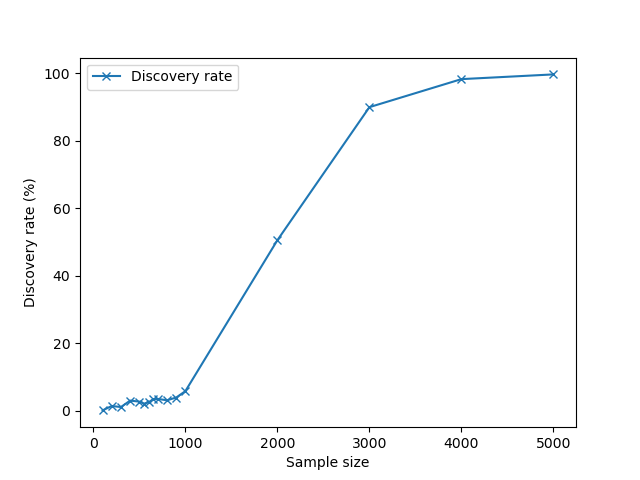
\includegraphics[width=\textwidth]{../plots/plot_f.png}
    \captionsetup{margin=1.3cm}
    \caption[width=0.2\pdfpagewidth]{Plot of the discovery rate as a function of the sample size (blue line), with error bars of 3 standard deviations. The red line shows the 90\% goal}
\end{figure}
\vspace{1\baselineskip}
Figure 5 shows that the discovery rate increases with the sample size, as expected. The simulation stops after it finds 3 sample sizes that have discovery rates above 90\%. Here, the minimum sample size appear to be around 800 samples, maybe 750. The error bars are set to represent 3 standard deviations from the mean. Here, it is clear that for 800 samples, there is a large proportion of the discovery rate distribution above the 90\% threshold. One note to make is that the intervals, when near the boundaries at 0 and 100\%, do cross over for 3 standard deviations. This means that the coverage of those intervals are not to be taken at face value. In reality, since no discovery rate could possibly be below 0\% or above 100\%, the discovery rate distributions are likely assymetric in those cases, and the uncertainties should as well. For these cases, other methods of confidence interval calculation may be used for accurate coverage, such as the Feldmann-Cousins method\cite{PhysRevD.57.3873}. 

\vspace*{1\baselineskip}

\underline{For (g):}

\vspace*{1\baselineskip}
For this simulation, seen in Figure 6, the discovery rate stays low for much longer than in (f). And the minimum sample size is much larger, at around 3500 samples.

\begin{figure}[htb]
    \centering
    \includegraphics[width=\textwidth]{../plots/plot_g.png}
    \captionsetup{margin=1.3cm}
    \caption[width=0.2\pdfpagewidth]{Plot of the discovery rate as a function of the sample size (blue line), with error bars at 3 $\sigma$. The red line shows the 90\% goal}
\end{figure}

\newpage
Comparing the 2 simulations, discerning 2 signals may be much harder to do than simply detect that there is one. This is seen especially when looking at a plot of the 2$^{nd}$ simulation's p.d.f.

\begin{figure}[htb]
    \centering
    \includegraphics[width=\textwidth]{../plots/plot_pdf_g.png}
    \captionsetup{margin=1.3cm}
    \caption[width=0.2\pdfpagewidth]{Plot of the total p.d.f.\ of the model, signal, and background, normalised for $M\in{[5,5.6]}$.}
\end{figure}

One can see the 2nd signal is much smaller than the first, making it harder to detect for smaller sample sizes. In other words, for smaller samples, the 2nd signal is more likely to be hidden in the background, or the 2 signals can be confused as one wider signal. Overall, since the discovery threshold is quite high, it is likely the p-values obtained are still significant enough to reject the null hypothesis for smaller samples. 
\newpage
\subsubsection*{Discussion}
Hence, the simulation shows that the minimum sample size for which the signal is discovered at least 90\% of the time is around 750-800 samples. This is a reasonable result, considering the size of the signal component (Figure 2). For the 2nd simulation, the minimum sample size is slightly above 3000 samples. This increase in required sample size can be the size and location of the 2nd signal component (Figure 5)


\bibliographystyle{plain}
\bibliography{refs.bib}


\section*{Appendix}

\subsection*{Use of generative AI}
Copilot's autocompletion feature was used in coding the project, when writing docstrings for the functions, and when covering repetitive parts of the code, like part (f) and (g)'s hypothesis testing.
ChatGPT was used to help in debugging the code, by providing the tracebacks when an error was difficult to understand.

\subsection*{README file}

\subsubsection*{Description} 
This repositery contains the code and written report for the S1 PDS coursework. The aim was to demonstrate the applications of statistical methods, including coding them.

\subsubsection*{Contents}  
Inside this \texttt{tmb76/} directory, there are 3 sub-directories to explore. One is the code directory (\texttt{src/}), which contains all the code used to generate the results and plots. The other is the plots directory (\texttt{plots/}), which contains all the plots generated by the code. An important note is that the plots direcotry will be created by the code if it does not exist yet. So if there is no plots direcotry in the repository yet, running all the code should lead to creating and filling one. The last one is the report directory, which contains the \LaTeX\ file for the report, as well as the pdf version of it. More importantly, there are an \texttt{environment.yml} file and a \texttt{Dockerfile}, which uses it, and one is advised to use.

\subsubsection*{How to run the code}
For permissions reasons, the \texttt{Dockerfile} is not set up to pull the repository directly as it builds the image. Therefore, one must first pull this repository to their local machine and then are free to build the Docker image from the \texttt{Dockerfile}.
All code can be run from the command line as follows:

\vspace*{1\baselineskip}
\begin{lstlisting}[language=bash, caption={Running the code for each part}]
    $ python src/solve_part_*.py
\end{lstlisting}

where * can be letters c through to g.  

Additionally, there is a \texttt{ndof\_for\_part\_f\_g.py} file which covers determining the appropriate number of degrees of freedom to be used in parts (f) and (g) (cf.\ part (f) and (g)'s code). This is also in the \texttt{src/} directory, and can therefore be run in a similar fashion:  

\vspace*{1\baselineskip}
\begin{lstlisting}[language=bash, caption={Running the number of DoF fitting code}]
    $ python src/ndof_for_part_f_g.py
\end{lstlisting}

Relevant outputs will be printed by the code to the terminal, and any plots generated will be saved to a \texttt{plots/} directory, that will get created if it doesn't exist yet.

This can all be done within a Docker container, by building an image from the \texttt{Dockerfile}, and running a container from it. 

From there, all files can be run in the same manner as above.


Note on time: The codes for part (c) to part (e) should each take less than a minute to run. For part (f), the code should take less than 5 minutes, with part (g) taking a little longer at The \texttt{ndof\_for\_part\_f\_g.py} is one of the more time consuming files to run, and could take around 10-15 minutes to run. This is based on running all of these on a MacBook Air M2 (2022, Ventura 13.2.1), with 8 GB of Memory.



\end{document}
